\chapter{Rezultate}
\label{chap:ch5}

În acest capitol se vor discuta și observa exemple din viața reală, atât exemple în care fiecare componentă lucrează corect, cât și situații în care un nod din pipeline a scos rezultate inexact pentru a evidenția atât parțile pozitive, cât si cele negative.

Dat fiind faptul că testarea sistemul bazat pe Raspberry Pi este dependent de un monitor, dispozitive periferice cum ar fi mouse și tastatură, dar și o sursă de curent ce poate livra 5.1 Volți cu 5 Amperi, combinație ce se găsește rar pe piață, colectarea de date este anevoiasă. Din acest motiv, pentru Raspberry Pi s-a testat un singur scenariu, care este comparat cu sistemul bazat pe platforma NVidia. În fiecare secțiune se va discuta atât platforma NVidia testat independent, cât și în comparație cu Raspberry Pi.

Pentru sectiunile: \ref{sec:ch5sec1}, \ref{sec:ch5sec2}, \ref{sec:ch5sec3}, testarea se va face strict din punct de vedere vizual, bazat pe imagini din timpul rulării. Pentru ultima secțiune se vor compara date metrice. 

\section{Aproximarea Adâncimii}
\label{sec:ch5sec1}

Imaginile captate au fost realizate în urma unui proces în care s-a aplicat un filtru inferno asupra hărții de adâncimi, în care punctele apropiate au fost colorate închis, iar cele indepartate în culori aprinse. 

În timpul testării platformei bazată pe NVidia, s-a constat că aproximarea adâncimilor este realizată cu succes, în diverse scenarii, atât interioare cât și exterioare. În următoarele exemple se pot observa următoarele rezultatele vizuale: \ref{fig:exterior_estimare}, \ref{fig:interior_estimare}.

\begin{figure}[htbp]
    \centering
    % Prima imagine (stânga)
    \begin{minipage}{0.48\textwidth}
        \centering
        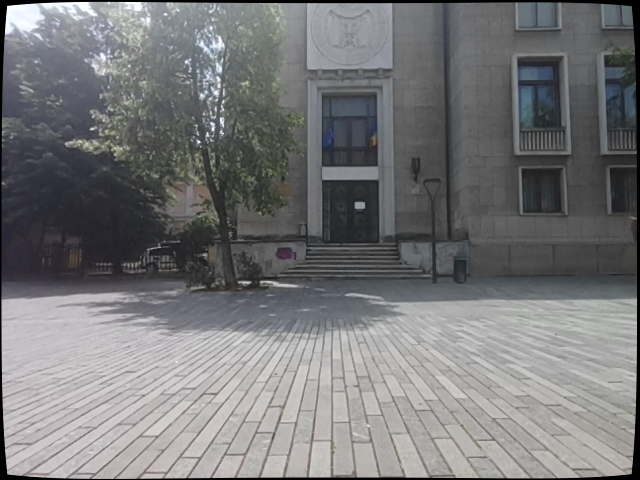
\includegraphics[width=\linewidth]{figures/real_world_examples/nvidia/20260604_114449_1_original.png}
        \caption{Imagine exteriroară captată după aplicării corecției.}
        \label{fig:exterior_original}
    \end{minipage}
    \hfill % Adaugă spațiu elastic între cele două imagini
    % A doua imagine (dreapta)
    \begin{minipage}{0.48\textwidth}
        \centering
        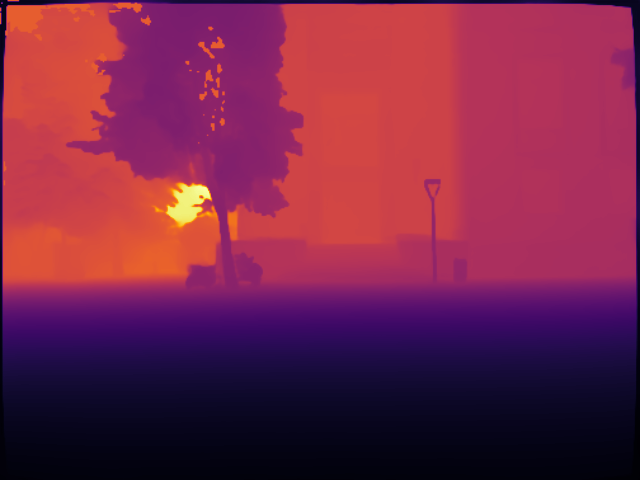
\includegraphics[width=\linewidth]{figures/real_world_examples/nvidia/20260604_114449_2_depth.png} % Schimbă cu numele imaginii tale
        \caption{Aproxamiare a adâncimi bazată pe imagine.}
        \label{fig:exterior_depth}
    \end{minipage}
    \caption{Comparație între imaginea orginilă și matricea de adâncime într-un scenariu exterior.}
    \label{fig:exterior_estimare}
\end{figure}

\begin{figure}[htbp]
    \centering
    % Prima imagine (stânga)
    \begin{minipage}{0.48\textwidth}
        \centering
        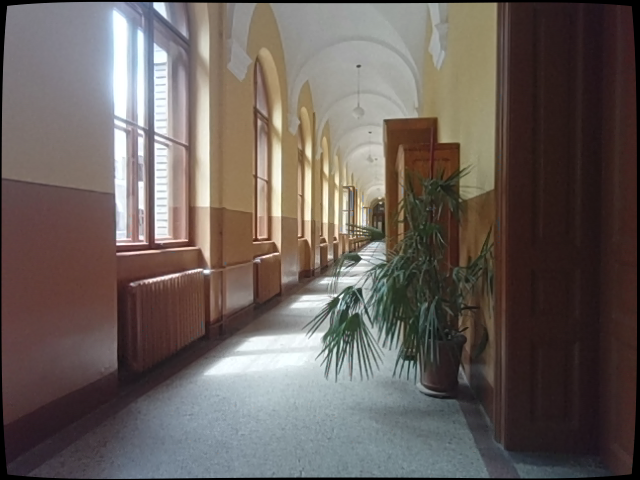
\includegraphics[width=\linewidth]{figures/real_world_examples/nvidia/20260604_115839_1_original.png}
        \caption{Imagine interioară captată după aplicării corecției.}
        \label{fig:interior_original}
    \end{minipage}
    \hfill % Adaugă spațiu elastic între cele două imagini
    % A doua imagine (dreapta)
    \begin{minipage}{0.48\textwidth}
        \centering
        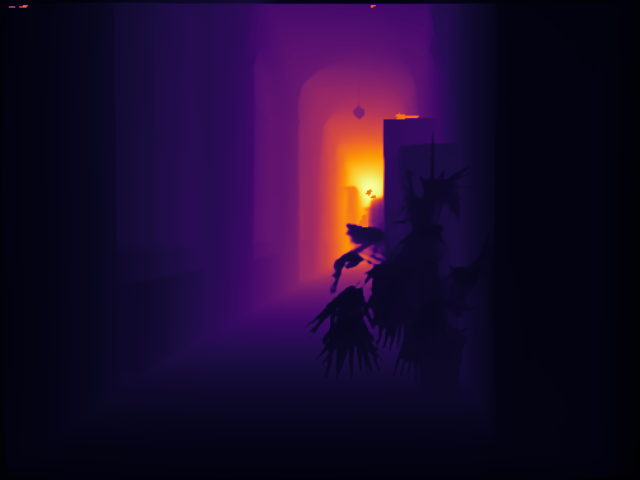
\includegraphics[width=\linewidth]{figures/real_world_examples/nvidia/20260604_115839_2_depth.png} % Schimbă cu numele imaginii tale
        \caption{Aproxamiare a adâncimi bazată pe imagine.}
        \label{fig:interior_depth}
    \end{minipage}
    \caption{Comparație între imaginea orginilă și matricea de adâncime într-un scenariu interior.}
    \label{fig:interior_estimare}
\end{figure}

Ținând cont că platforma bazată pe Raspberry Pi este limitată în putere, și modelul este atât cu o generație mai slab, cât și numărul de parametrii este mai mic, ne aștăm ca rezultatele sa fie mai slabe, și ele întradevăr sunt, dar mai degrabă când vine vorba de previzia muchiilor. Comparând matricea estimării cu imaginea orginilă se pot remarca elementele pe care le-a destins \ref{fig:interior_estimare_rpi}.

\begin{figure}[htbp]
    \centering
    % Prima imagine (stânga)
    \begin{minipage}{0.48\textwidth}
        \centering
        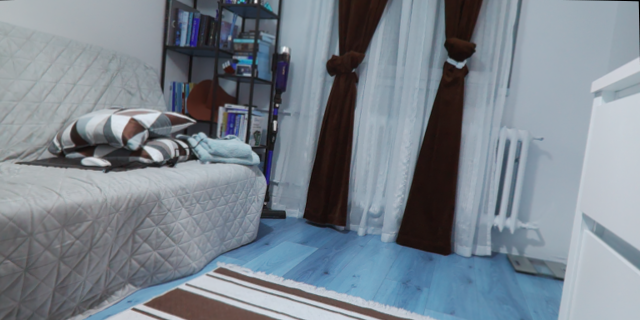
\includegraphics[width=\linewidth]{figures/real_world_examples/rpi/20260608_224242_1_original.png}
        \caption{Imagine interioară captată după aplicării corecției folosind Raspberry Pi + Hailo-8.}
        \label{fig:interior_original_rpi}
    \end{minipage}
    \hfill % Adaugă spațiu elastic între cele două imagini
    % A doua imagine (dreapta)
    \begin{minipage}{0.48\textwidth}
        \centering
        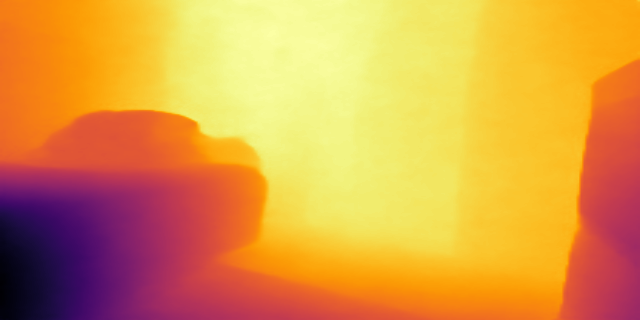
\includegraphics[width=\linewidth]{figures/real_world_examples/rpi/20260608_224242_2_depth.png} % Schimbă cu numele imaginii tale
        \caption{Aproxamiare a adâncimi bazată pe imagine folosind Raspberry Pi + Hailo-8.}
        \label{fig:interior_depth_rpi}
    \end{minipage}
    \caption{Comparație între imaginea orginilă și matricea de adâncime într-un scenariu interior folosind Raspberry Pi + Hailo-8.}
    \label{fig:interior_estimare_rpi}
\end{figure}

\section{Detecția Solului}
\label{sec:ch5sec2}

În majoritatea cazurile, detecția solului determină planul bine așa cum se poate vedea în figura \ref{fig:good_example_sol}.

\begin{figure}[htbp]
    \centering
    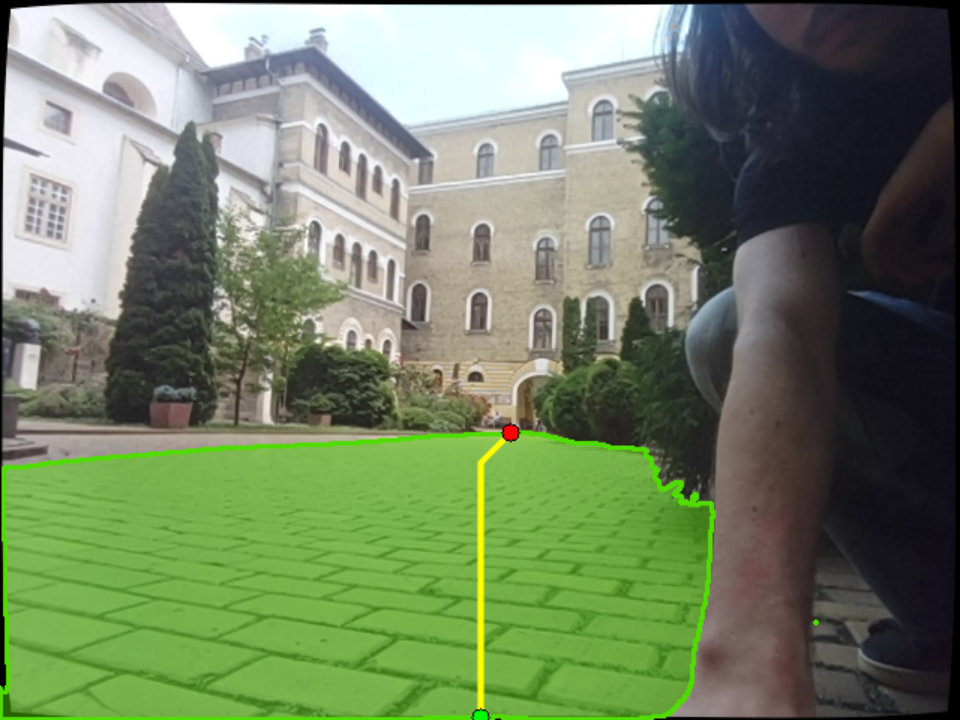
\includegraphics[width=0.8\linewidth]{figures/real_world_examples/nvidia/20260604_115437_5_view.png}
    \caption{Exemplu în care detecția solului detectează solul așa cum ne așteptăm.}
    \label{fig:good_example_sol}
\end{figure}

Cu toate acestea, s-a observat că pe traseele lungi nu sunt cuprinse în totalitatea, însemnând că sistemul nu detectează punctele distante ca facând parte din planul detectat al solului \ref{fig:long_road_example_sol}. Este greu de găsit un o explicație pentru acest fenomen, întrucât matricea adâncimi, din punct de vedere vizual, pare precisă așa cum se poate vedea în figura \ref{fig:long_road_example_sol_depth}. Mai multe studii pe acest fenomen trebuie efectuate.

\begin{figure}[htbp]
    \centering
    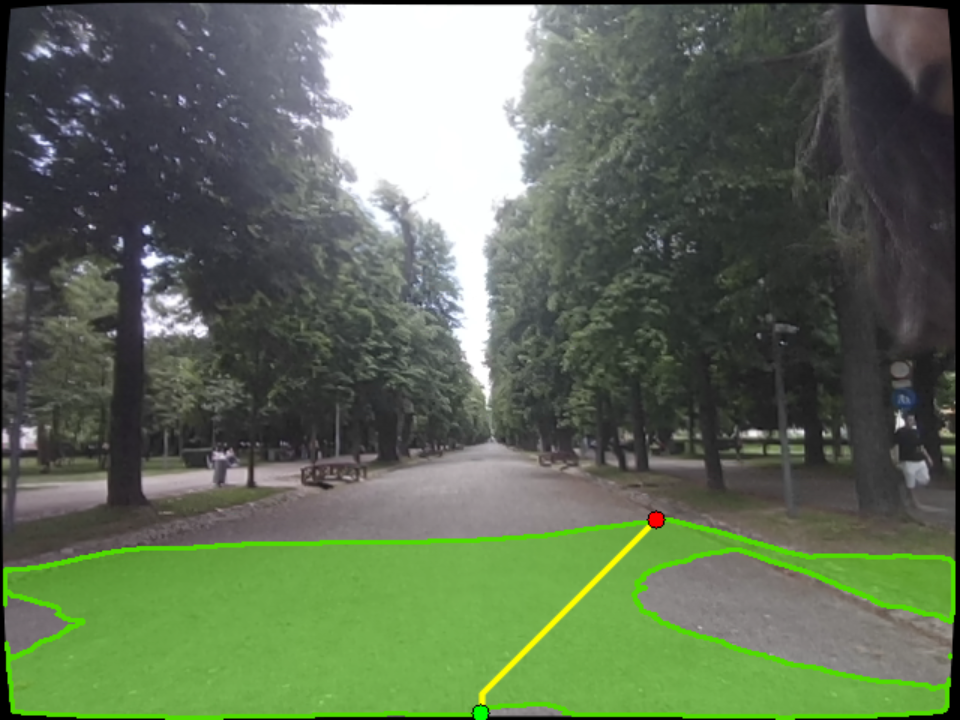
\includegraphics[width=0.8\linewidth]{figures/real_world_examples/nvidia/20260604_125553_5_view.png}
    \caption{Exemplu în care detecția solului nu detectează solul în totalitate.}
    \label{fig:long_road_example_sol}
\end{figure}

\begin{figure}[htbp]
    \centering
    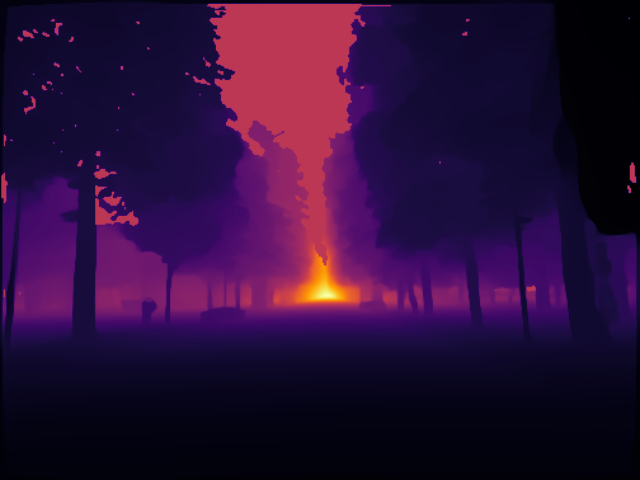
\includegraphics[width=0.8\linewidth]{figures/real_world_examples/nvidia/20260604_125553_2_depth.png}
    \caption{Matricea adâncimii pentru exemplul anterior.}
    \label{fig:long_road_example_sol_depth}
\end{figure}

O limitare majoră a metodei de detecție a solului aleasă pentru acest sistem stă tocmai în natura metodei. Pe scurt, detectează planul în care majoritatea punctelor din matricea de adâncime se află. Statistic vorbind, în majoritatea cazurilor acel plan este planului solului, însă în spații înguste acest fapt nu se mai aplică, iar planul solului este detectat greșit, așa cum se poate vedea în figura \ref{fig:small_space_sol}.

\begin{figure}[htbp]
    \centering
    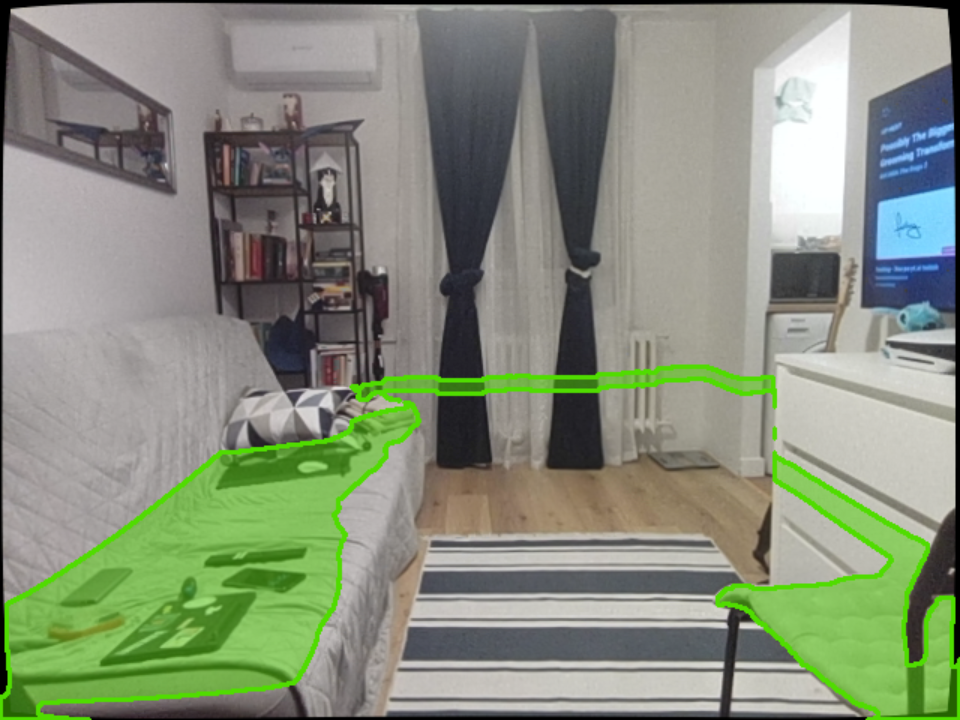
\includegraphics[width=0.8\linewidth]{figures/real_world_examples/nvidia/20260608_225109_5_view.png}
    \caption{Exemplu în care planul solului este detectat greșit datorită spațiului îngust.}
    \label{fig:small_space_sol}
\end{figure}

Totodată, s-a observat că în unele situații, sistemul detectează planul de mers cu porțiuni goale \ref{fig:spatii_sol}. Această problemă poate fi atribuită matricii de adâncime. 

\begin{figure}[htbp]
    \centering
    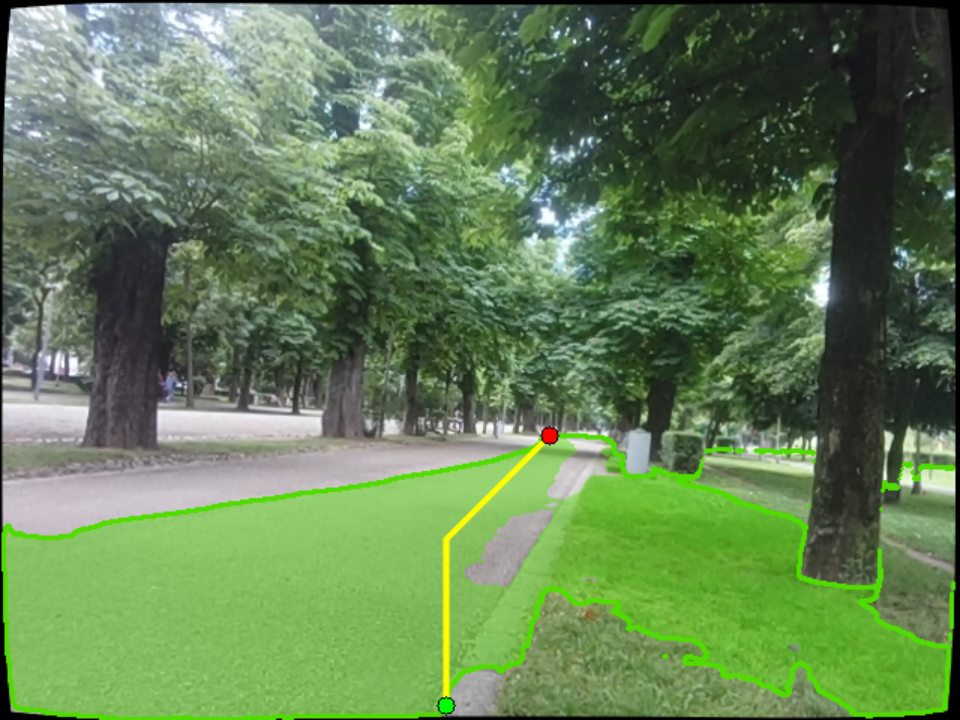
\includegraphics[width=0.8\linewidth]{figures/real_world_examples/nvidia/20260604_125945_5_view.png}
    \caption{Exemplu în care planul solului nu este detectat în întregime.}
    \label{fig:spatii_sol}
\end{figure}

Până în acest moment, toate aceste exemple au fost bazate de sistemul bazat pe NVidia. Comparând sistemul bazat pe nvidia vs. Raspberry Pi, se poate observa cum calitatea și precizia matricii de adâncimi influențează detecția solului, întrucât Raspberry Pi nu a reușit să detecteze solul precis, așa cum se poate vedea în figura \ref{}.

\begin{figure}[htbp]
    \centering
    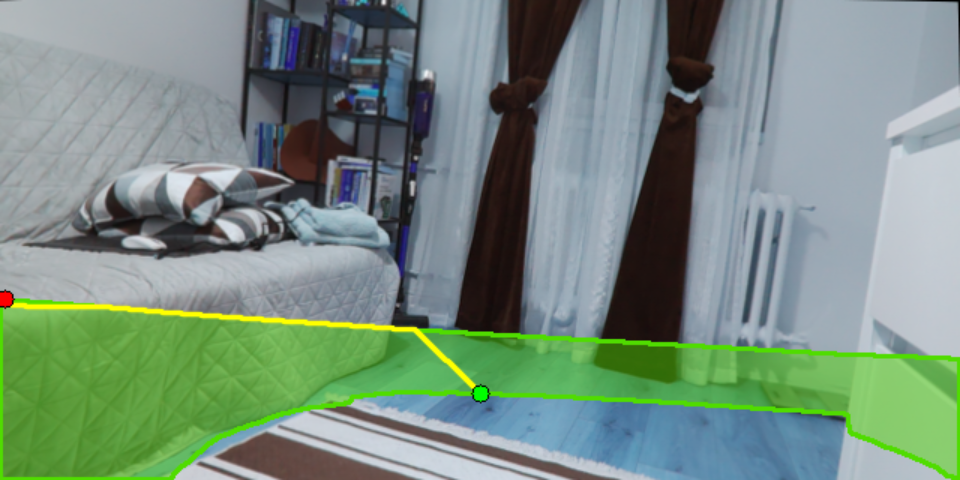
\includegraphics[width=0.8\linewidth]{figures/real_world_examples/rpi/20260608_224242_5_view.png}
    \caption{Exemplu în care Raspberry Pi-ul eșuează în a detecta solul.}
    \label{fig:rpi_sol}
\end{figure}

O altă limitare majoră este faptul că nu face distincția dintre un trotuar și o stradă circulată de mașini. Această metodă de determinare a solului a fost aleasă datorită vitezei de precosare superioară comparată cu metodele ce folosesc rețele neuronale, dat fiind scopul inițial de a construi un sistem compact, cu un buget relativ mic, și limitări hardware semnificative.

\section{Determinarea Drumului de Cost Minim}
\label{sec:ch5sec3}

Drumul de cost minim nu este găsit pe proiecția în 3D a planului de mers, dar mai bine zis pe proiecția lui în 2D. Acest lucru nu garantează că mereu se va găsi drumul de cost minim din viața reală, însă de cele mai multe ori este suficient.

\section{Latență}
\label{sec:ch5sec4}

Spre deosebire de secțiunile anterioare, evaluarea latenței se bazează pe date metrice colectate de modulul de profilare integrat în aplicație. Acesta măsoară, cu ajutorul funcției \texttt{time.perf\_counter()}, durata fiecărei etape a pipeline-ului pentru fiecare cadru procesat și o înregistrează într-un fișier CSV, în loturi, pentru a nu introduce întârzieri suplimentare pe calea critică. Statisticile prezentate în continuare au fost obținute pe platforma bazată pe NVidia (rezoluție 640$\times$480, model Depth Anything 3 metric, varianta Large), agregând aproximativ 9.989 de cadre din 13 sesiuni de rulare distincte. Primul cadru al fiecărei sesiuni a fost exclus, întrucât include inițializarea modelului și nu reflectă regimul normal de funcționare.

Pipeline-ul este compus din patru etape sincrone — corecția distorsiunii, estimarea adâncimii, detecția solului și determinarea drumului — a căror sumă constituie timpul total de procesare per cadru. Capturarea cadrului de la cameră se desfășoară pe un thread separat, în paralel cu procesarea, motiv pentru care nu este inclusă în timpul total, deși este raportată informativ. Rezultatele agregate sunt prezentate în tabelul \ref{tab:latenta_nvidia}.

\begin{table}[htbp]
    \centering
    \begin{tabular}{lcccc}
        \toprule
        Etapă & Medie & Mediană & Dev. std. & p95 \\
              & [ms] & [ms] & [ms] & [ms] \\
        \midrule
        Capturare cadru$^{*}$ & 34,1 & 32,1 & 4,0 & 42,4 \\
        Corecția distorsiunii & 0,5 & 0,5 & 1,7 & 0,7 \\
        Estimarea adâncimii & 64,1 & 64,1 & 9,1 & 69,5 \\
        Detecția solului & 0,9 & 0,9 & 0,3 & 1,1 \\
        Determinarea drumului & 47,7 & 13,7 & 200,9 & 212,3 \\
        \midrule
        Total procesare & 113,2 & 79,6 & 200,9 & 276,6 \\
        \bottomrule
    \end{tabular}
    \caption{Statistici de latență per etapă pe platforma NVidia, agregate peste 9.989 de cadre din 13 sesiuni de rulare (cadrul de inițializare exclus). $^{*}$Capturarea cadrului se execută pe un thread separat și nu este inclusă în timpul total de procesare.}
    \label{tab:latenta_nvidia}
\end{table}

După cum se poate observa, estimarea adâncimii domină timpul de procesare, reprezentând aproximativ 56\% din total (64,1 ms în medie). Aceasta este, de altfel, singura etapă bazată pe o rețea neuronală și constituie gâtuirea (\textit{bottleneck}) sistemului, fiind totodată foarte stabilă, cu o deviație standard de doar 9,1 ms. Prin contrast, etapele pur geometrice — corecția distorsiunii și detecția solului — sunt neglijabile, fiecare sub 1 ms, fapt ce confirmă decizia de proiectare de a folosi o metodă bazată pe RANSAC pentru detecția solului în locul unei a doua rețele neuronale.

Etapa de determinare a drumului prezintă un comportament aparte: în mod tipic este ieftină (mediană de 13,7 ms), însă distribuția sa are o coadă grea — aproximativ 19\% dintre cadre depășesc 50 ms, iar în cazuri degenerate căutarea drumului poate dura câteva secunde. Acest fapt explică diferența semnificativă dintre medie (47,7 ms) și mediană și se reflectă în cei doi indicatori ai cadenței: pornind de la mediana timpului total (79,6 ms) sistemul atinge aproximativ \textbf{12,6 cadre pe secundă}, în timp ce media (113,2 ms) corespunde unei valori de aproximativ \textbf{8,8 cadre pe secundă}. În practică, sistemul funcționează tipic în jurul valorii de 12 FPS, vârfurile ocazionale ale etapei de determinare a drumului cauzând micro-blocaje punctuale.

Pe platforma NVidia, performanța temporală este așadar mărginită de modelul de estimare a adâncimii, restul componentelor adăugând un cost redus și predictibil. O eventuală optimizare a latenței ar trebui să vizeze în primul rând accelerarea inferenței modelului de adâncime și, secundar, stabilizarea etapei de determinare a drumului în cazurile nefavorabile.

Pentru a evidenția impactul platformei hardware asupra latenței, aceleași măsurători au fost realizate și pe sistemul bazat pe Raspberry Pi + Hailo-8. Spre deosebire de platforma NVidia, aici estimarea adâncimii este delegată acceleratorului neuronal Hailo-8 și folosește un model mult mai mic — Depth Anything 2, varianta ViT-S, la rezoluția 224$\times$224, în mod relativ. Statisticile, agregate peste aproximativ 2.086 de cadre din 2 sesiuni de rulare, sunt prezentate în tabelul \ref{tab:latenta_rpi}.

\begin{table}[htbp]
    \centering
    \begin{tabular}{lcccc}
        \toprule
        Etapă & Medie & Mediană & Dev. std. & p95 \\
              & [ms] & [ms] & [ms] & [ms] \\
        \midrule
        Capturare cadru$^{*}$ & 59,1 & 53,9 & 32,2 & 122,8 \\
        Corecția distorsiunii & 3,8 & 3,3 & 5,3 & 7,1 \\
        Estimarea adâncimii & 42,3 & 41,8 & 1,8 & 45,7 \\
        Detecția solului & 6,1 & 5,6 & 2,2 & 10,4 \\
        Determinarea drumului & 83,4 & 36,7 & 105,4 & 226,3 \\
        \midrule
        Total procesare & 135,5 & 90,8 & 104,8 & 277,7 \\
        \bottomrule
    \end{tabular}
    \caption{Statistici de latență per etapă pe platforma Raspberry Pi + Hailo-8, agregate peste 2.086 de cadre din 2 sesiuni de rulare (cadrul de inițializare exclus). $^{*}$Capturarea cadrului se execută pe un thread separat și nu este inclusă în timpul total de procesare.}
    \label{tab:latenta_rpi}
\end{table}

Rezultatele relevă o inversare a profilului de latență față de platforma NVidia. Dacă acolo gâtuirea o constituia estimarea adâncimii, pe Raspberry Pi această etapă devine una dintre cele mai rapide (42,3 ms în medie, sub valoarea de pe NVidia și remarcabil de stabilă, cu o deviație standard de doar 1,8 ms), tocmai datorită modelului mult mai mic rulat pe NPU-ul dedicat. În schimb, gâtuirea se mută pe etapa de determinare a drumului (83,4 ms în medie, aproximativ 61\% din total), care se execută pe procesorul ARM, semnificativ mai lent decât GPU-ul plăcii NVidia. Această etapă prezintă din nou o coadă grea, peste 43\% dintre cadre depășind 50 ms. Trebuie subliniat însă că latențele estimării adâncimii nu sunt direct comparabile din punct de vedere calitativ, întrucât cele două platforme rulează modele diferite ca generație și dimensiune, așa cum s-a discutat în secțiunea \ref{sec:ch5sec1}.

În ansamblu, cele două platforme ating cadențe surprinzător de apropiate — aproximativ 11,0 cadre pe secundă (mediană) pe Raspberry Pi față de 12,6 pe NVidia — însă din motive diferite: sistemul NVidia este mărginit de inferența unui model de adâncime puternic, în timp ce sistemul Raspberry Pi, deși descarcă inferența pe NPU, este mărginit de calculele geometrice efectuate pe procesorul ARM. Această observație sugerează că, pe platforma embedded, optimizarea ar trebui să vizeze în primul rând etapa de determinare a drumului, complementar față de direcția indicată pentru platforma NVidia.
